\section{Použití trezoru}
První nasazení trezoru na akci pořádané Robotárnou \parencite{robotarna} proběhlo na příměstském robotickém táboře v srpnu roku 2019.
Jednalo se o první variantu trezoru, která kdy spatřila světlo světa (viz kapitola \ref{E1-vyvoj}). Tábor trval pět dní a děti dostaly první tři dny na stavbu mechaniky a poslední dva dny 
se~programovalo. 

Trezor tehdy sklidil úspěch a tak započal vývoj dalších verzí, které už byly specializovanější (viz kapitoly \ref{E2-vyvoj} a  \ref{E3-vyvoj}) a přidal se vývoj i mechanických
variant (jsou popsané v kapitolách \ref{M1-vyvoj}, \ref{M2-vyvoj} a \ref{M3-vyvoj}).

\paragraph{Trezor ve volnočasových kurzek robotiky}
Další používání trezoru pro\-bí\-ha\-lo ve volnočasovém kurzu robotiky, který jsem spoluvedl, a účastníci v~něm stavěli nejprve tehdy aktuální mechanickou variantu, verzi M2 (popsaná v kapitole \ref{M2-vyvoj}).
Protože účastníci kurzu byli vetšinou již docela zkušení, jednalo se u nimi téměř jen o \uv{rozcvičku}, kterou měli za několik kroužků hotovou a následovala stavba trezoru E3. 

Bohužel kvůli pandemickým opatřením si ne všichni účastníci stihli trezor E3 postavit a vůbec jsme se nedostali k programování, natož aby jsme si s~trezorem zorganizovali nějakou herní akci, 
jak bylo dříve v plánu.

\paragraph{Trpasličí trezor}
Chvíli po té, co vznikl trezor M3 \ref{M3-vyvoj} \ref{M3-popis},  proběhla první akce s trezorem, která nebyla pod taktovkou Robotárny. Zároveň to byla také 
první akce, na které se trezor nestavěl a jen se využíval.

Protože na akci byly menší děti, byl trezor místo klasické číselné stupnice  vybaven obrázkovým kódem, jak je vidět na obrázku \obr{fig:M3-trpaslici}. %todo co se tam s tím trezorem dělalo 

Toto však byla poslední akce která se stihla uskutečnit před započetím pandemických opatření.

\begin{figure}[htbp]
    \centering
    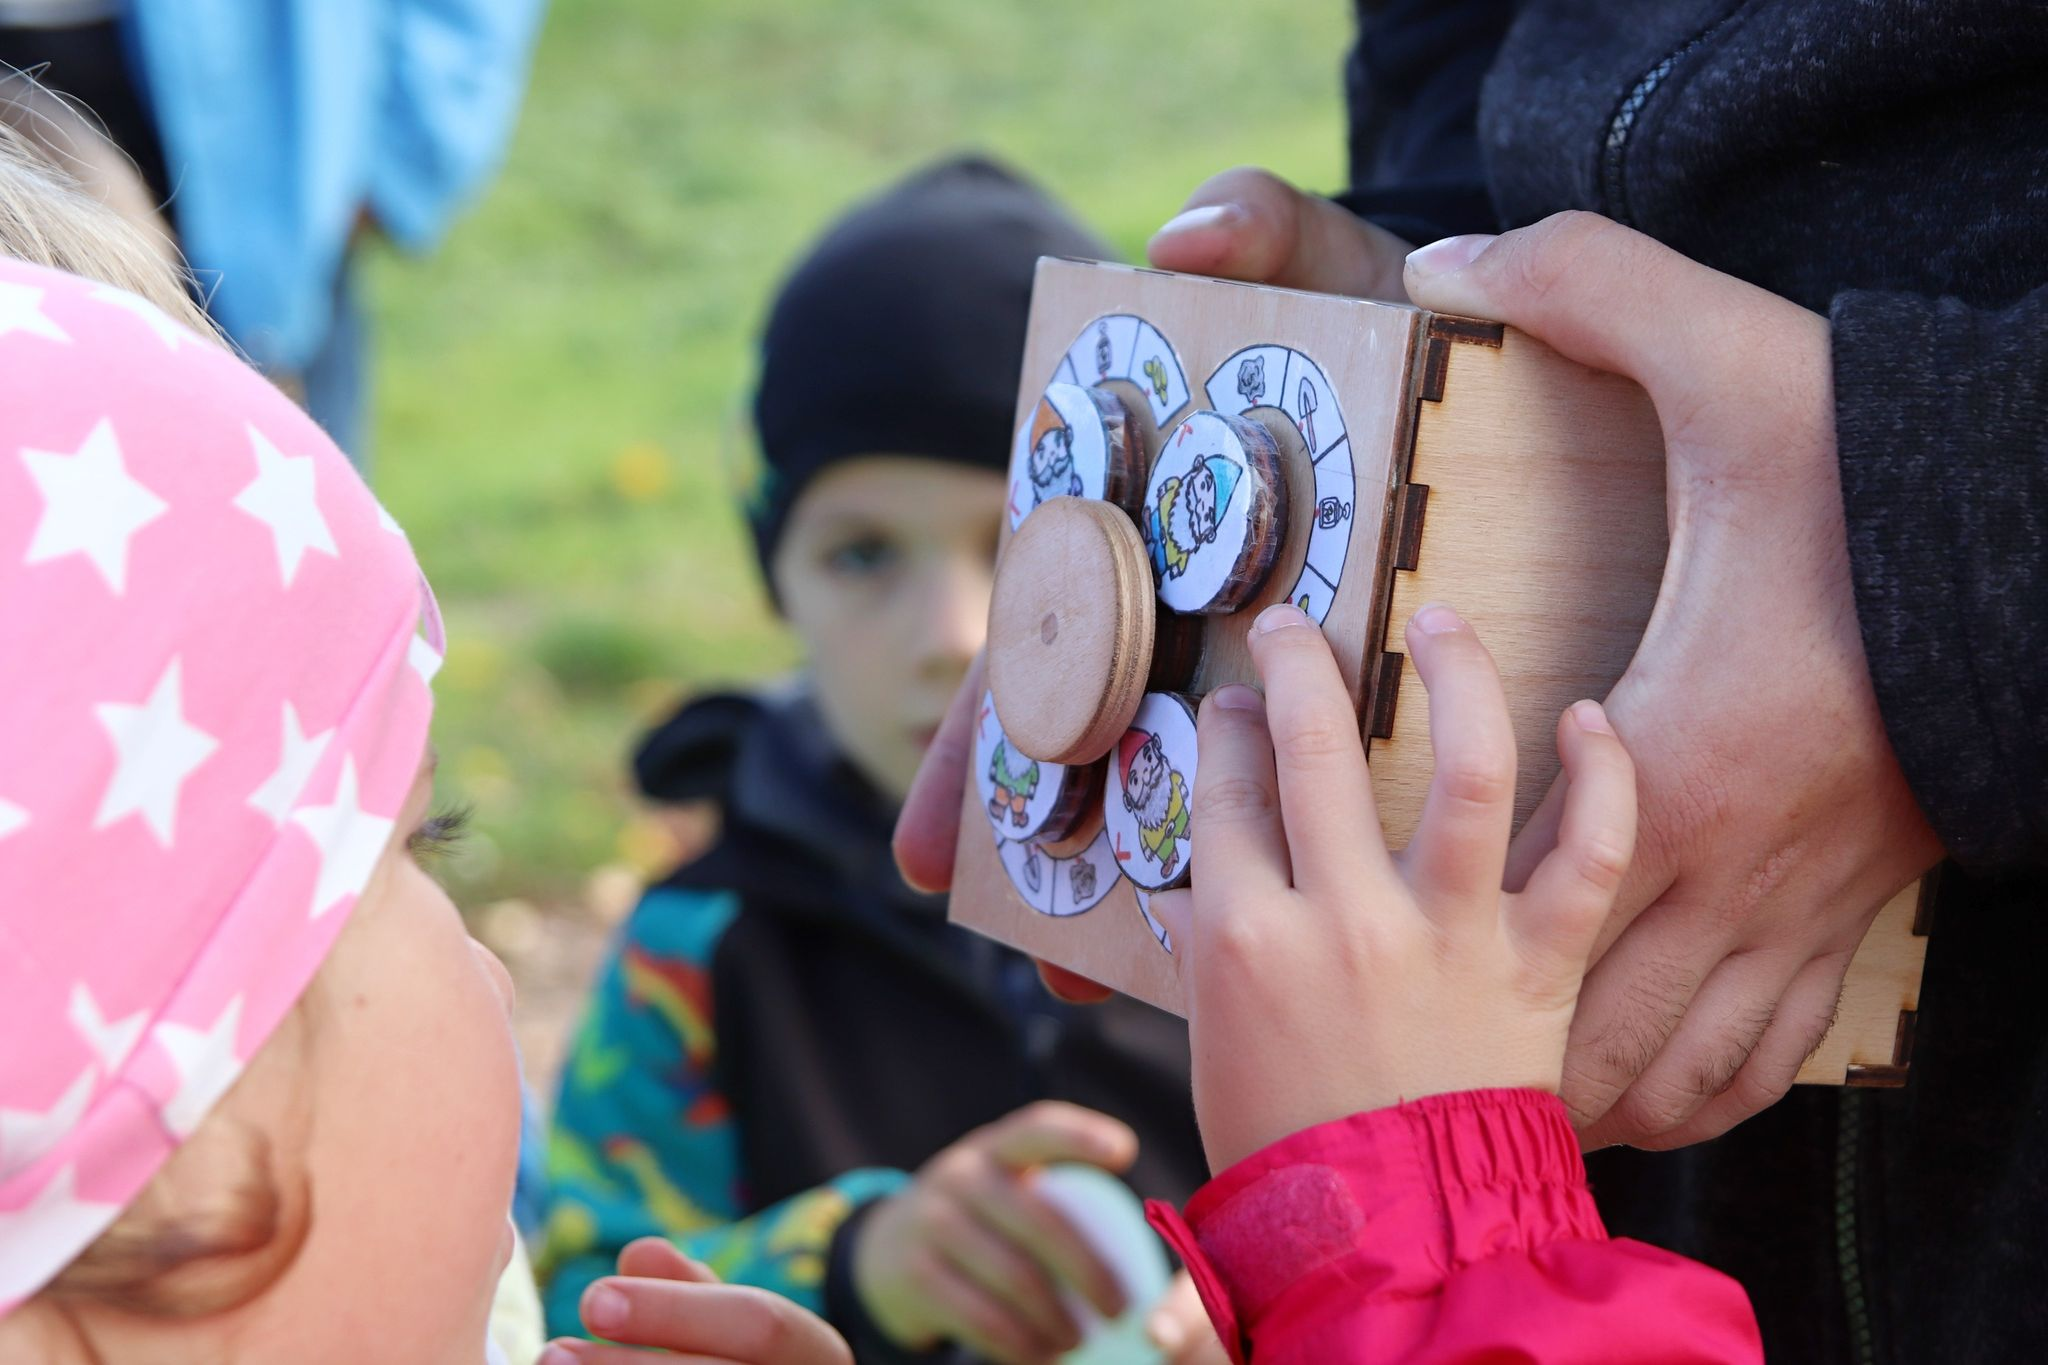
\includegraphics[width=\textwidth]{kapitoly/obrazky/M3/trpaslici.png}
    \caption{Trpasličí trezor}
    \label{fig:M3-trpaslici}
\end{figure}

%todo další akce nikdy moc nebyli v plánu, prostě se už počítalo s lockdownem takže se ani nic nevymýšlelo (bavil jsem se s Jirkou že mi vyrobí nějakej ten papír)